% !TeX encoding = UTF-8
% !TeX spellcheck = en_US
% !TeX root = ../MasterThesis_OlivierChurlaud_2016.tex

\chapter{Mathematical appendices}
\section{Brightness and brilliance}
\label{apx:brightness_brilliance}
In the following section, the $\theta$ subscript is either $x$ or $y$.

The quality of the beam is described by the \emph{brightness} and the \emph{brilliance}.

Let F be the \emph{flux} of photons, normalized to a beam current of 1~A
\begin{equation}
F = \frac{\text{photons}}{\text{s 0.1\% BW A}},
\end{equation}

The brightness describes the angular divergence of the beam (given by $\sigma_\theta'=\sqrt{\frac{\varepsilon_\theta}{\beta_\theta}}$). It is defined as:
\begin{equation}
S = \frac{F}{2 \pi \sigma'_x \sigma'_y} = \frac{F \sqrt{\beta_x \beta_y}}{2 \pi \sqrt{\varepsilon_x \varepsilon_y}} = \frac{\text{photons}}{\text{s 0.1\% BW mrad$^2$ A}}
\end{equation}
while the brilliance includes also the transverse dimensions ($\sigma_\theta=\sqrt{\varepsilon_\theta \beta_\theta}$):
\begin{equation}
B = \frac{F}{4 \pi^2 \sigma_x \sigma_y \sigma'_x \sigma'_y} = \frac{F}{4 \pi^2 \varepsilon_x \varepsilon_y} = \frac{\text{photons}}{\text{s 0.1\% mm$^2$ BW mrad$^2$ A}}
\end{equation}

These definitions vary in literature. These are taken from the book of K.~Wille~\cite{book:wille}, and apply to Gaussian-shaped electron beams. The invariant idea is that both values are determinated by the beam emittance $\sigma$: the design of the accelerators and the correction are aimed at obtaining the smallest emittance $\varepsilon_\theta$ as possible.

\section{Principal components analysis -- Karhunen-Loève transform (KLT)}
\label{apx:KLT}

Let $\mat{X}$ be a signal with n dimensions.

\begin{equation}
\mat{X} = \left[
\begin{array}{@{}c|c|c|c@{}}
&&&\\ \vec{X}_1 & \vec{X}_2 & \dots & \vec{X}_n \\ &&&
\end{array}
\right]
\end{equation}

The covariance matrix is extracted
\begin{equation}
\mat{A} = \text{covar}(X)
\end{equation}
and diagonalized so that the eigenvalues are sorted in a decreasing order (the first one being the most significant). The covariance being symmetric, it is always diagonalizable in $\mathbb{R}$.
\begin{equation}
\mat{D} = \mat{P}^{t} \mat{A} \, \mat{P}
\end{equation}

The principal components are the columns of
\begin{equation}
\hat{\mat{X}} = \mat{P}^{t} \mat{X}
\end{equation}
and in the first column of the matrix resides the most significant of theses principal components.

\chapter{mBox++}
\label{apx:mbox}
The program that was handling the correction computation (see \cref{sec:correction_sa_technical}) was written in \textsc{Matlab}. It had 2 main drawbacks:
\begin{itemize}
    \item it was not very fast. \textsc{Matlab} being an interpreted language, it produces slower programs than a compiled one such as C or C++.
    \item it was difficult to extend. The code was written in a very functional way, making it hard to had debugging outputs, timers or other modules. If this can be done in \textsc{Matlab}, it is however not the easiest programming language to do it.
\end{itemize}

The program was thus rethought and rewritten from scratch. It can be found at
\begin{center}
    \url{https://github.com/ochurlaud/MSc_FOFB-mBox},
\end{center} 
licensed with the GNU General Public License v2.

\section{Specifications}

\subsection{Constrains}
\begin{itemize}
    \item mBox++ must work without any change in the current architecture and environment
    \item mBox++ must be easily maintainable and improved: modularized, encapsulated and namespaced code (e.g. object oriented) is needed (global scope must not be used too much to be able to trace variable evolutions)
\end{itemize}

\subsection{Performance}
\begin{itemize}
    \item mBox++ must be able to provide the same results as the \textsc{Matlab} version, and better in extended modes
    \item mBox++ must be at least as fast as the \textsc{Matlab} version
    \item mBox++ must be robust (e.g. graceful exit when requested, no crash on error/exception)
\end{itemize}

\subsection{Features}
\begin{itemize}
    \item mBox++ must have a \textit{read only} mode where it computes the correction but has no influence on the environment
    \item mBox++ must provide an experimental mode (where the correction is handled by external scripts)
    \item mBox++ must be able to communicate with external programs and to share its data.
    \item Tools to debug/profile must be provided
\end{itemize}

\section{Technology used}

\subsection{Language and paradigm used}
\begin{description}
    \item[Technology:] C++, Standard Template Library (STL)
    \item[Rationale:] Compiled language, thus faster than \textsc{Matlab} or Python. It is higher level than C and thus more manageable. It supports and eases object oriented programming, which allows encapsulation and to organize the code in business objects (e.g. one class is called \textit{Logger} and deals with the logs and debug strings, another acquire the data and is called \textit{ADC}..). Every needed types exist in the STL (vectors, strings, etc.) and it is a widely used library very well documented and time tested. The C++\,11 version is used as it provides several improvements compared to previous ones and is now available on most platforms.
    \item[Resources:] \url{http://www.cplusplus.com} --- \url{http://en.cppreference.com}
\end{description}

\subsection{Algebra computation}
\begin{description}
    \item[Technology:] Armadillo
    \item[Rationale:] Open source C++ library whose API is close to \textsc{Matlab}'s and supports multi-thread calculation. It is a long tested technology (currently version 7.x) with a large and active scientific community.
    \item[Resources:] \url{http://arma.sourceforge.net}
\end{description}

\subsection{External communication}
\begin{description}
   \item[Technology:] ZeroMQ\footnote{ZeroMQ is often shortened as zmq or ZMQ}
   \item[Rationale:] Multi-platform, multi-language and open source distributed messaging library. It can be used to share messages between Python, Matlab, C/C++. It is a long tested technology (currently version 4.x), with a large and active community
   \item[Resources:] \url{http://zeromq.org}
\end{description}

\subsection{Others}
\begin{itemize}
\item The program should be able to execute interpreted scripts: it uses the official Python library in C to call Python script. 
\item To ease the localization of dependency and the compilation, the CMake (\url{https://cmake.org}) build tool is used.
\end{itemize}

\section{The program: architecture and runtime scheme}

\Cref{fig:mbox_class_diag} represents the UML\footnote{Unified Modeling Language: modeling language intended to provide a standard way to visualize the design of a system (Wikipedia)} diagram of the classes that build mBox++.

\begin{sidewaysfigure}
    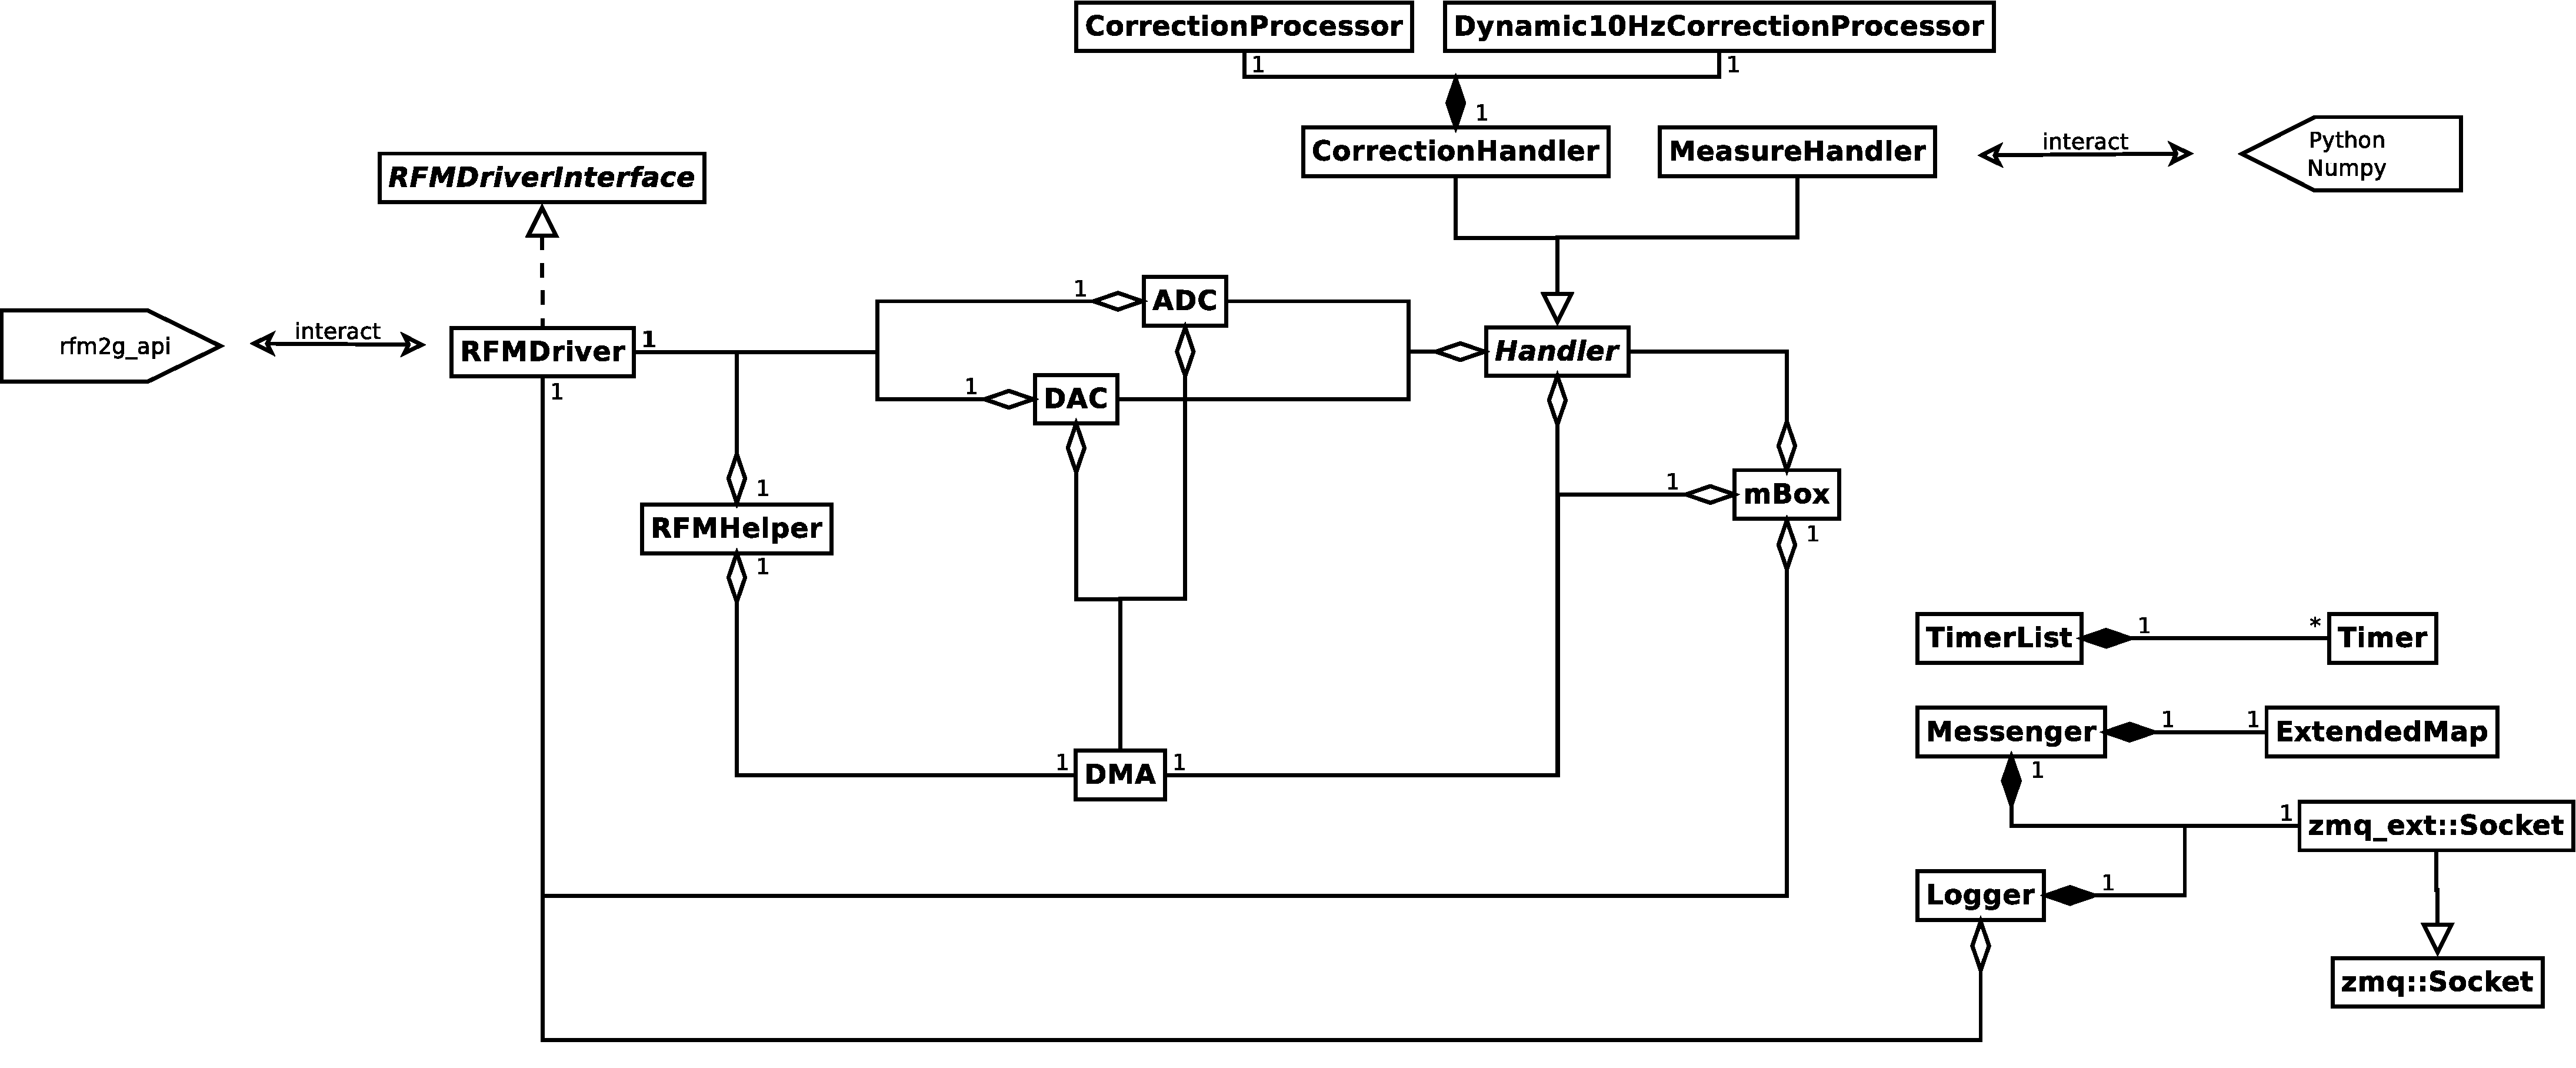
\includegraphics[width=\linewidth]{img/mBox_classDiagram}
    \caption{\label{fig:mbox_class_diag}Class diagram of the mBox++ program}
\end{sidewaysfigure}

The class \texttt{mBox} is the one from which everything begins. It creates the shared objects and deals with the state machine process. It owns a \texttt{Handler} which can be a \texttt{CorrectionHandler} if mBox++ runs in normal mode, or a \texttt{MeasureHandler} if it runs in experiment mode.

The actual mathematics (computation of the calculation) happens in the processors. If the handler is a \texttt{CorrectionHandler}, then the processor can be a \texttt{CorrectionProcessor} which does exactly what the \textsc{Matlab} code did (see \cref{sec:correction_state_of_art}) or a \texttt{Dynamic10HzCorrectionProcessor} which implements what was described in \cref{sec:dyn_corr_ex_10Hz}. Otherwise, if the handler is a \texttt{MeasureHandler}, the processor is directly the Python script provided by the user.

A handler delegates the actions to objects it owns:
\begin{enumerate}
    \item The \texttt{ADC} reads the data from the ADC reserved area in the RFM.
    \item The handler reads the data from the \texttt{ADC} object, does some conversions (mostly from a integer representation to doubles) and provides the data to its processor that calculates the correction.
    \item The correction is then converted to integers by the handler and provided to the \texttt{DAC} which writes it to the DAC reserved area in the RFM.
\end{enumerate}

To access the RFM, the C functions provided by the constructor are used. An interface \texttt{RFMDriverInterface} is implemented by the \texttt{RFMDriver} which provides a more object oriented version of the C~API.

\remark In order to be able to test the program without having access to a RFM hardware, a second \texttt{RFMDriver} (accessible by compiling with the \texttt{-DDUMMY\_DRIVER=ON} flag) implements the interface: it reads and writes in a 64~Mb binary file that represents the RFM. This can allow the creation of a simulation of the whole environment and expedient interaction with the program..

Three modules are statically constructed and globally defined (in their own namespaces):
\begin{itemize}
    \item \texttt{TimerList} which is a "clever" list of \texttt{Timer}s, used to profile the parts of the code. A new or already existing timer can be started with
     \begin{c++}
         TimingModule::addTimer("name_of_timer");           
     \end{c++}
    stopped with 
    \begin{c++}
        TimingModule::timer("name_of_timer").stop();   
    \end{c++}
    and its values shown (in this case once every 1000 times) with
    \begin{c++}
        TimingModule::printAll(Timer::Unit::ms, 1000);
    \end{c++}
    The \texttt{TimimgModule} being global, it can be accessed from everywhere and thus some profiling can be done across objects and functions.

    \item \texttt{Logger} which is a class logging actions and errors. By defaults, errors only are shown to the stdout (standard output stream). Logs and errors are published on a given port (3333 by default) with ZeroMQ and can be read by subscribed services (the logs and errors can thus be output, saved in a file, published on a website stream or whatever crazy idea the user can have). It uses the ZeroMQ Publisher mode. A debug mode is also available (see \texttt{--help} command). It publishes incoming and outgoing values that can be used by other scripts or programs for display, scripting, value-checking... The full description of the uses are given in the Doxygen\footnote{Popular documentation generator that extracts specific comments to produce PDF or HTML documentation. See \url{http://www.stack.nl/~dimitri/doxygen/index.html}} documentation
    
    \item \texttt{Messenger} which is a class for exchanging information with outside scripts and programs. It is listening on a given port (3334 by default). It is using the ZeroMQ Router mode. Every time it receives a request, it processes it and either returns the value of the requested variable, or sets the given variable to the received value. The difference with the \texttt{Logger} is that the logger publishes values even if no one is listening and sends it when asked by the code, whereas the \texttt{Messenger} only answers queries. It is notably used in the harmonic correction process described in \cref{sec:dyn_corr_ex_10Hz}: a python script calculates all the phases and amplitudes and sends the outcome, which are then used by \texttt{Dynamic10HzCorrectionProcessor}.
\end{itemize}

\section{Project organization}
The project is organized as followed:
\begin{itemize}
    \item \texttt{/cmake} contains CMake modules to find other libraries and dependencies.
    \item \texttt{/doc} contains resources for the documentation and the generated documentation (which is not synchronized in the version control).
    \item \texttt{/experimentScripts} contains Python scripts that can be used as processor in experiment mode.
    \item \texttt{/python\_tools} contains Python scripts and modules that can be used with the program: the helper for the harmonic correction is there (\texttt{tenHz.py}), a module to communicate with mBox++ through a binary file in dummy mode (\texttt{cbox.py}, \texttt{dummy\_simul.py}) and various helpers to subscribe to the ZeroMQ streams, save data in a specified way...
    \item \texttt{/src} contains all the C++ code to be compiled. Its root contains the core of the project. The rest of the code is split in \texttt{/src/modules}, \texttt{/src/handlers} for a better readability.     
    \end{itemize}
Finally at the root of the project is \texttt{README.md} file giving the dependencies, how to compile, install and use mBox++. A Doxygen configuration file \texttt{doxygen.conf} let the documentation be generated by starting
\begin{verbatim}
    $ doxygen doxygen.conf
\end{verbatim}
   
\section{Use}
mBox++ cannot run if it does not receive the order from the cBox: it would otherwise hang in a waiting state.
It can be used in normal mode
\begin{verbatim}
    $ mbox --rw
\end{verbatim}
in read only
\begin{verbatim}
    $ mbox --ro
\end{verbatim}
A full overview of the commands are given by
\begin{verbatim}
    $ mbox --help

    === mbox (2015-2016) ===
    Use:
    mbox --ro
        Read only version: just reads the RFM and calculates
        the correction, don't write it back.
    mbox --rw
        Read-write version: reads the RFM, calculates the
        correction and write it on the RFM.
    mbox --experiment <FILENAME>
        Read-write version for experiments: read the file <FILENAME>
        to know which values to create.
    
    Other arguments (to append):
    --debug
        Print the logs on the the stderr.
    --logport <PORT>
        Which port the log publisher should use.
    --queryport <PORT>
        Which port the query messenger should use.
\end{verbatim}

\chapter{Search Kick}
Search Kick was originally only able to find kicks in the orbit, in order to localize perturbation sources. It is currently closer to a Python orbit toolbox that allows translating dump data between various formats, localizing perturbations, and other small algorithms for inverting matrices or optimizing signals.

The library can be found at 
\begin{center}
        \url{https://github.com/ochurlaud/MSc_SearchKicks}
\end{center}
licensed with the GNU General Public License v2.


    